\documentclass{article}
\setlength{\parskip}{5pt} % esp. entre parrafos
\setlength{\parindent}{0pt} % esp. al inicio de un parrafo
\usepackage{amsmath} % mates
\usepackage[sort&compress,numbers]{natbib} % referencias
\usepackage{url} % que las URLs se vean lindos
\usepackage[top=25mm,left=20mm,right=20mm,bottom=25mm]{geometry} % margenes
\usepackage{hyperref} % ligas de URLs
\usepackage{graphicx} % poner figuras
\usepackage[spanish]{babel} % otros idiomas
\usepackage[utf8]{inputenc}
\author{Elías Alejandro García Bueno \\
Bryan Alejandro Andrade Amaya \\ Jesus Adalberto Mendoza Flores} % author
\title{Tarea 2} % titulo
\date{\today}

\begin{document} % inicia contenido

\maketitle % cabecera

\begin{abstract} % resumen
Una prótesis es un sustituto artificial de una parte del cuerpo faltante (tanto en singular como en plural; se llama prótesis).
Existen muchos tipos diferentes de prótesis. Algunas se usan por fuera del cuerpo y pueden ponerse y quitarse (prótesis externas) y otras se insertan durante una cirugía (implantes).
\end{abstract}

\section{Introducción}\label{intro} % seccion y etiqueta

La mano es un órgano que conforma las extremidades del cuerpo humano para la manipulación Física del medio, la cual se encuentra en los extremos de los antebrazos. Permite realizar ciertos trabajos como tomar y maniobrar un objeto, la comunicación por medio de gestos y no solo en individuos que usan el lenguaje de señas, por otro lado, las personas que tienen discapacidad visual las manos serian una herramienta muy útil para hacer uso del sistema Braille.
Día a día en cualquier parte del mundo se encuentran casos en que el ser humano está expuesto a sufrir mutilaciones debido a los accidentes de trabajo, conflictos, enfermedades y malformaciones que generan amputaciones.  Estas situaciones traen como secuela que la pérdida de manos que genera la reducción de su capacidad para realizar distintas funciones debido a que 166 una gran parte de su habilidad se reduce a la hora de agarrar y maniobrar objetos específicos. Igualmente, generando incomunicación gestual y visual, es decir las personas que sufren de discapacidad a la hora de ver y hablar. Para este problema la solución viable es la implementación de una prótesis, siendo esta, un instrumento que permite reemplazar el miembro carente  Esta prótesis es desarrollada con el objetivo de reemplazar  una  parte, una  función  o  un  miembro completo del cuerpo humano alterado  Permitiendo al afectado   recuperar   parte de la movilidad, el funcionamiento, el aspecto y el agarre




%\\begin{figure} % figura
%    \centering
%    \includegraphics[width=150mm]{output3.jpg} % archivo
%    \caption{resultados del programa}
%    \label{grafica}
%\end{figure}

\section{Desarrollo}
\cite{chavez2014diseno}\textbf{La mano humana}

\item Es el órgano primordial para la manipulación del medio que nos rodea. Los dedos son algunas de las zonas con más sensibilidad; además son la principal fuente de interacción y comunicación con el entorno, es por eso que el sentido del tacto, a pesar de poder realizarse con todo el cuerpo, se relaciona directamente con la mano. Está estructurada por un complicado y muy relacionado sistema de huesos, ligamentos, tendones que flexionan y otros que extienden, músculos intrínsecos con sus respectivos tendones, vasos y nervios. No obstante, además de ser un órgano para efectuar tareas, es un receptor sensible preciso e importante. La mano humana tiene una forma claramente plana y ancha. La palma se conforma de piezas o eminencias que rodean un hueco. La eminencia tenar se forma por cuatro músculos, los cuales están reservados al movimiento del dedo pulgar; la hipotenar se instala desde arriba y hacia adentro de la palma; la inferior es conocida como eminencia de los dedos, se encuentra apartada por el pliegue dígito palmar y el surco de flexión de los cuatro dedos. En el hueco de la mano se perciben tres pliegues: superior, medio e inferior, cortados por un pliegue longitudinal; estos cuatro pliegues trazan una “M” recubierta por membranas de tejidos fibrosos entrecruzados, conocidos como aponeurosis que envuelven a los músculos.

El miembro superior cuenta con un total de veintisiete huesos, distribuidos ocho en la región del carpo esqueleto de la muñeca, cinco huesos metacarpianos delgados y ligeramente alargados que ocupan toda la palma de la mano y catorce falanges subclasificadas en cinco falanges distales, cuatro medias y cinco proximales (Andrei, Correa, & Pareja, 2012)
Las medidas antropomórficas de la mano según la norma DIN 33 402.2° parte (Melo, 2013), son promedio de una mano real adulta y se muestran en la figura 2.
\vspace{5mm}


\begin{figure} % figura
    \centering
    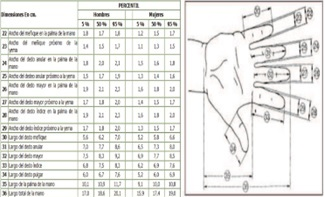
\includegraphics[width=100mm]{dimensiones.jpg} % archivo
    \caption{Dimensiones promedio de la mano}
    \label{grafica}
\end{figure}


{\textbf{Análisis de las Propiedades de los Materiales}}

Para realizar prótesis se consideran aspectos tales como la resistencia del material, su peso y su costo. Básicamente una prótesis Transhumeral, cuenta con tres secciones, el encaje, el polímero que sostiene el mecanismo, y la mano robótica, misma que tiene un acabado estético (Fernández, 2007\\
El encaje es la parte que conecta al cuerpo con la prótesis y es el único componente que tiene contacto directo con él. Dentro de la variedad de materiales que se utilizan en la fabricación de encajes, se encuentran la fibra de carbón, el kevlar, polietileno y polipropileno; en la Tabla 1 se muestra una comparativa de algunas de sus propiedades físicas (Uellendahl, 1998). 


\item En el diseño de la mano robótica es necesario combinar rigidez y ligereza. Por esto muchos materiales de bajo peso son usados, sobre todo el aluminio que no es tan fuerte como otros metales pero que puede soportar el peso o fuerza requerido en las prótesis de mano. Desde el punto de vista físico, el aluminio puro (Association, Aluminum Standards and Data, 2006) posee una resistencia muy baja a la tracción y una dureza escasa. En cambio, unido en aleación con otros elementos, el aluminio adquiere características mecánicas muy superiores. A estas aleaciones se les conoce con el nombre genérico de Duraluminio, y pueden ser centenares de aleaciones diferentes. 

\item Otra alternativa para la construcción de una prótesis, es el Titanio, debido a que es muy fuerte y liviano, sin embargo es muy caro. Muchos componentes que antes se hacían de acero son actualmente elaborados de titanio. Comparte muchas características con el acero inoxidable. Puede formar aleaciones con otros elementos, tales como Hierro, Aluminio, Vanadio, Molibdeno y otros. Por último, el acero, es un material muy fuerte y resistente (AIMEN, 2005), sin embargo es relativamente pesado, por lo que no es la mejor opción en una prótesis. Debido a sus propiedades, se puede utilizar para fabricar componentes pequeños en donde importa más la fuerza del elemento para resistir fuerzas, que el diseño. Algunas partes de los dedos se fabrican de acero, pues son piezas pequeñas por lo que se utiliza poco material.

\begin{figure} % figura
    \centering
    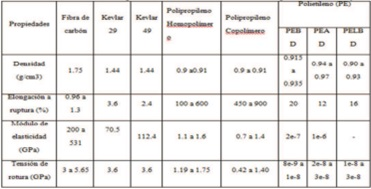
\includegraphics[width=90mm]{propiedades.jpg} % archivo
    \caption{Propiedades de los materiales para el encaje}
    \label{grafica}
\end{figure}


\begin{figure} % figura
    \centering
    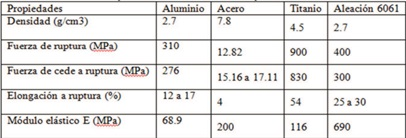
\includegraphics[width=90mm]{propiedades_protesis.jpg} % archivo
    \caption{Propiedades de los materiales para la mano robotica}
    \label{grafica}
\end{figure}

\cite{serrezuela2018diseno} {\textbf{Materiales y diseño ingenieril}}
\item {\textbf{Materialesl}}
\item Para el desarrollo del proyecto se utilizaron materiales como motores D.C., tarjeta Arduino Uno, nylon de poliácido láctico (PLA) para reemplazar el material acrilonitrilo butadieno estireno (ABS), conectores   y cableado eléctricos, tornillos, entre otros. En el caso del software, se usó SolidWorks para el diseño de la prótesis y LabVIEW para el sistema de control y algoritmos de trayectorias.

\item {\textbf{Diseño ingenieril}}
\item Una vez realizado la revisión bibliográfica de prótesis de manos robóticas antropomórficas subactuadas, se desarrolla la  perspectiva  teórica basada en los mecanismos de cuatro barras   Para ello se diseña el prototipo de mano en SolidWorks y se construye las piezas en la impresora Ultimaker3 Para  generar  los  algoritmos generadores  de trayectorias, se desarrolla la programación en LabVIEW  Estese interconecta con la tarjeta embebida Arduino, el cual a su vez tiene la función de generar las ordenes de control de los motores DC  Para lograr el correcto movimiento y por ende, el correcto funcionamiento del sistema, se realiza el análisis matemático de la cinemática directa e inversa de la mano en su totalidad   Así  mismo,  se  genera  simulaciones  en Matlab para encontrar el volumen de trabajo del sistema, y para validar el movimiento de cada una de las articulaciones de los dedos 3 Geometría  de  la mano  robótica  subactuada antropomórfica. En  esta parte precisaremos  la composición  física  de cualquiera de los dedos excepto el pulgar ya que para los dedos  índice,  medio,  anular  y  meñique  se  pude generalizar  

\section{Conclusiones}
Las prótesis han preexistido desde hace miles de décadas, no   obstante   su   desarrollo   se   ha   detenido aproximadamente por  la  misma  cantidad  de  tiempo. Escasamente   hace   pocos   períodos   se   emprendió   el verdadero ascenso en esta área.   Las prótesis de manos nos   permite tener un sobresaliente panorama con respecto a las  innovaciones    y  las  herramientas  con  las que necesitamos para la elaboración  la prótesis. Gracias   al   empleo   de   nuevas   herramientas   de desarrollo   de   hardware  y  software  se   pueden  crear nuevos  desarrollo  en  este  campo. \\ El desarrollo de sistemas automáticos de control en prótesis de manos que permitan recobrar la funcionalidad  parcial  de  esta  se convierte en un verdadero reto. En conclusión, la prótesis del futuro diferenciará un poco de  la  prótesis  ideal,  ya que    preexisten    limitaciones    que    dificultosamente lograrán ser superadas. No obstante la prótesis del futuro podrá proporcionar a la persona afectada la mayoría  de las funciones que la mano real puede brindar, como es el agarre de tipo cilíndrico, esférico y tipo pinza.




\bibliographystyle{plainnat}
\bibliography{bibliografia.bib}



\end{document}